\documentclass{standalone}
\usepackage{tikz}
\usepackage{ctex}
\setCJKmainfont{Noto Serif CJK SC}
\usepackage{chemmacros,siunitx}
\begin{document}
\small
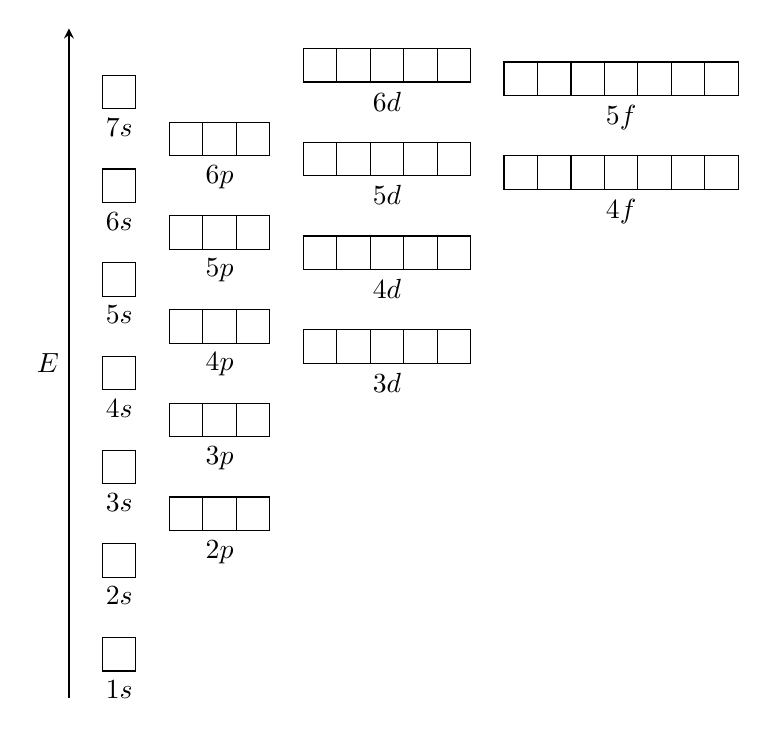
\begin{tikzpicture}[>=stealth,scale=.85]
  \foreach \y in {1,...,7}
  {
    \draw(0,1.4*\y)rectangle++(0.5,0.5);
    \node at (0.25,\y*1.4)[below]{$\y s$};
  }
  \foreach \y in {2,...,6}
  {
    \draw(1,\y*1.4+0.7)rectangle++(1.5,0.5);
    \draw(1.5,\y*1.4+0.7)--++(0,0.5)(2,\y*1.4+0.7)--++(0,0.5);
    \node at (1.75,\y*1.4+0.7)[below]{$\y p$};
  }
  \foreach \y in {3,...,6}
  {
    \draw(3,\y*1.4+1.8)rectangle++(2.5,0.5);
    \draw(3.5,\y*1.4+1.8)--++(0,0.5)
         (4,\y*1.4+1.8)--++(0,0.5)
         (4.5,\y*1.4+1.8)--++(0,0.5)
         (5,\y*1.4+1.8)--++(0,0.5);
    \node at (4.25,\y*1.4+1.8)[below]{$\y d$};
  }
  \foreach \y in {4,5}
  {
    \draw(6,\y*1.4+3.0)rectangle++(3.5,0.5);
    \draw(6.5,\y*1.4+3.0)--++(0,0.5)
         (7,\y*1.4+3.0)--++(0,0.5)
         (7.5,\y*1.4+3.0)--++(0,0.5)
         (8,\y*1.4+3.0)--++(0,0.5)
         (8.5,\y*1.4+3.0)--++(0,0.5)
         (9,\y*1.4+3.0)--++(0,0.5);
    \node at (7.75,\y*1.4+3.0)[below]{$\y f$};
  }
  \draw[->,semithick](-0.5,1)--(-0.5,11) node[midway,left]{$E$};
\end{tikzpicture}
\end{document}